\usepackage{dirtree}
\usepackage{listings}
\lstset{basicstyle=\ttfamily}

\usepackage{tikz}
\usetikzlibrary{graphs,graphdrawing,arrows.meta,positioning}
\usegdlibrary{trees}
\tikzset{branch/.style={green!70!black},tag/.style={yellow!85!black}}

\usetheme{Madrid}
\usecolortheme{seahorse}


\graphicspath{{./images/}}

%Use itemize rather than enumerate for \note[item].
%From https://tex.stackexchange.com/a/28969
\AtBeginNote{%
	\let\enumerate\itemize%
	\let\endenumerate\enditemize%
}

%A command for unnumbered footnotes.
%From https://tex.stackexchange.com/a/30723
\makeatletter
\def\blfootnote{\gdef\@thefnmark{}\@footnotetext}
\makeatother

%\vdots with appropraite spacing for use outside a matrix.
%From https://tex.stackexchange.com/a/112212
\makeatletter
\DeclareRobustCommand{\rvdots}{%
	\vbox{
		\baselineskip4\p@\lineskiplimit\z@
		\kern-\p@
		\hbox{.}\hbox{.}\hbox{.}
	}}
\makeatother

\title{An Introduction to Git}
\author{Christopher Brown}
\date{}

\begin{document}

\begin{frame}
	\titlepage
	
	\note[item]{
		I'm going to teach this over several sessions.
		Hopefully the first session will teach enough to just spin up a Git repository and start making commits.
		But if that's all you ever do, you're missing out on most of the benefits that version control will give you.
		So subsequent sessions will focus on how to get the most out of Git, and use it to be more productive.
	}
\end{frame}

\part{Prerequisites}

\begin{frame}
	\partpage
	
	\note[item]{
		Before we start looking at Git, there're some prerequisites we need to go over.
		
		\item
		Primarily, you'll need to know the very basics of the shell.
		We'll use Git from the command line (the shell), so it'll help to be familiar with it.
		
		\item
		There're also a few other things I'll explain the details of now, to save having to go off on tangents later.
	}
\end{frame}

\section{The Shell}

\subsection{Introduction}

\begin{frame}{Which Shell?}
	\begin{itemize}
		\item \texttt{sh}: the Bourne Shell by Stephen Bourne, 1977
		\item \texttt{bash}: the Bourne Again SHell, 1989
		\item \texttt{zsh}, \texttt{ksh}, \texttt{tcsh}, \texttt{rc}\dots
	\end{itemize}
	\texttt{bash} is default on most Linux distros.
	
	Mac OS X defaults to \texttt{zsh}.
	
	Git on Windows comes with a \texttt{bash} emulator.
	
	\note[item]{
		You might have heard of the shell called the ``terminal'' or the ``command line''.
		It's a text-based interface to your computer.
		You can use it instead of a graphical user interface (GUI).
		
		\item
		There are GUIs for Git, but it's good to know how to use it through the command line.
		
		\item
		Different shells, \texttt{bash}, \texttt{zsh}, etc.\ are mostly based on the Bourne shell.
		There are differences, but they're all similar enough that we shouldn't run into the differences here.
		
		\item
		On Linux or Mac OS X, you should be able to search for and open the ``terminal''.
		On Windows, you're looking for ``Git Bash''.
		Open it now.
	}
\end{frame}

\subsection{Navigation}

\begin{frame}{UNIX Directories}
	\begin{itemize}
		\item \texttt{/} is the root directory
		\item \texttt{cd \textasciitilde} is your user's home directory
		\begin{itemize}
			\item \texttt{/home/abc123/} on Linux
			\item \texttt{/Users/abc123/} on Mac OS X
			\item \texttt{/c/Users/abc123/} in Git Bash on Windows
		\end{itemize}
		\item \texttt{.} is the current directory
		\item \texttt{..} is the parent directory
	\end{itemize}
	Paths starting with \texttt{/} or \texttt{cd \textasciitilde} are \emph{absolute paths}.
	
	Others are \emph{relative paths}, and start from the current directory.
	
	\note[item]{
		The first thing to learn is how the directory structure is represented on the command line.
		Directories and files have \emph{paths}: a list, one inside the other, of the directories in the tree structure reaching down to them.
		Paths are separated by forward slashes.
		Windows sometimes uses backslashes, but Git Bash does it properly with forward slashes.
		
		\item
		The difference between absolute and relative paths is important in general.
		Generally, your code should use relative paths whenever possible.
		This is especially important in Git repositories.
		Suppose someone else downloads your repo: they'll have a different username, or put it in a different place, so the absolute path will be different.
		Use relative paths instead.
	}
\end{frame}

\begin{frame}{Moving Around}
	\begin{itemize}
		\item \texttt{pwd}: Print Working Directory
		\item \texttt{cd}: Change Directory
		\begin{itemize}
			\item \texttt{cd -} goes to previous directory
		\end{itemize}
		\item Right click in file manager to open command line there
	\end{itemize}
	
	\note[item]{
		At any point, your shell is in one directory: the \emph{working directory}.
		\texttt{pwd} (print working directory) will tell you which directory you're in.
		Try it now.
		
		\item
		Before we start doing anything, we'll usually want to move to the correct directory.
		We do this with \texttt{cd} (change directory).
		
		\item
		\texttt{cd} can take a relative or absolute path.
		This is when \texttt{..} to go up a directory becomes useful, and note that we can chain this or include it mid-path.
		\texttt{cd} can also take the special argument \texttt{-} to go back to the most recent working directory.
		Play around with it.
		
		\item
		You can also open the command line directly in a directory, by right-clicking in the file manager.
	}
\end{frame}

\subsection{Inspection}

\begin{frame}{Looking Around}
	\begin{itemize}
		\item \texttt{ls}: LiSt directory contents
		\begin{itemize}
			\item \texttt{ls -a} includes hidden files/directories (e.g.\ \texttt{.git}, {.gitignore})
			\item \texttt{ls -l} gives extra info
			\item \texttt{ls -al} does both
		\end{itemize}
	\end{itemize}
	
	\note[item]{
		When you're in a directory, you want to know which files are there.
		Or which directories, so you can \texttt{cd} further in.
		\texttt{ls} tells you.
		
		\item
		\texttt{ls} takes options, a.k.a. \emph{flags}.
		\texttt{-a} (all) shows hidden files and directories, which start with a dot.
		This is important, 'cause Git uses these.
		\texttt{-l} (long) shows owner, permissions, size, date, etc.
		
		\item
		A hyphen and a single letter is the convention for flags in the shell.
		We can combine options by giving them sequentially.
		A single hyphen followed by multiple letters also combines flags.
		Order doesn't matter.
		Demonstrate this.
		
		\item
		Some programs take long options: these use two hyphens followed by a word.
		We'll see these later on some Git commands.
	}
\end{frame}

\begin{frame}{Looking at Files}
	\begin{itemize}
		\item \texttt{cat}: print a file
		\item \texttt{head}: print the first 10 lines of a file
		\item \texttt{tail}: print the last 10 lines of a file
		\item \texttt{less}: open a file in the pager
	\end{itemize}
	
	\note[item]{
		There are a variety of ways we can look at the contents of a file in the command line.
		These all work within the command line, so they'll only work for text files.
		
		\item
		The names are a bit funny.
		\texttt{cat} comes from ``concatenate'', because it can print several files back-to-back.
		\texttt{less} is a better version of \texttt{more}.
	}
\end{frame}

\begin{frame}{Opening Files \& Directories}
	\begin{itemize}
		\item Open a file with the OS:
		\begin{itemize}
			\item \texttt{open} on Mac OS X
			\item \texttt{xdg-open} in Linux
			\item \texttt{start} in Git Bash on Windows
		\end{itemize}
		\item Using these on a directory opens the file manager
	\end{itemize}
	
	\note[item]{
		If you want to use your normal text editor, or work with non-text files, you can open files as though you'd double-clicked them in your file manager.
		How to do this differs by OS.
		
		\item
		You can also use these to open your file manager, which can be helpful to move or copy files if you're not familiar with doing so on the command line.
	}
\end{frame}

\subsection{Modification}

\begin{frame}{Changing Things}
	\begin{itemize}
		\item \texttt{mkdir}: MaKe DIRectory
		\item \texttt{rmdir}: ReMove empty DIRectory
		\item \texttt{touch}: create blank file, or change last modified date
		\item \texttt{cp}: CoPy a file
		\begin{itemize}
			\item \texttt{cp -r}: CoPy a directory (recursive)
		\end{itemize}
		\item \texttt{mv}: MoVe/rename a file/directory
		\item \texttt{rm}: ReMove a file
		\begin{itemize}
			\item \texttt{rm -i} asks confirmation: safer
			\item \texttt{rm -r} removes a directory and everything inside: DANGER!
		\end{itemize}
	\end{itemize}
	
	\note[item]{
		We can use all sorts of commands to create, remove, copy, or remove files or directories.
		I won't go into the details now, and you should be able to do most of this with your file manager.
		But this might be useful in future, and you might see me using these out of habit.
	}
\end{frame}

\section{Hashes}

\subsection{SHA1}

\begin{frame}{Hashing}
	\centering
	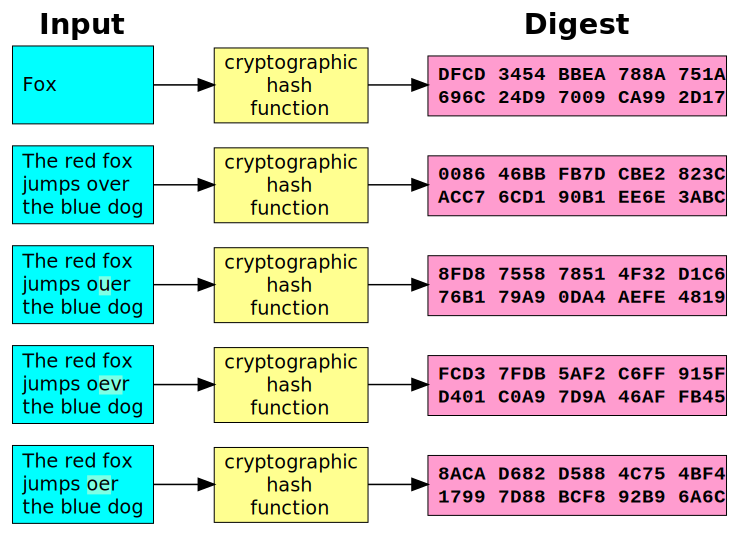
\includegraphics[width=\textwidth,height=0.8\textheight,keepaspectratio]{sha1}
	\blfootnote{Cryptographic Hash Function by Jorge Stolfi}
	
	\note[item]{
		A hash function converts some arbitrary input to a fixed-length string of seemingly-random input.
		It always converts the same input to the same output.
		But small changes in input cause large changes in output.
		
		\item
		This example uses the SHA1 hash function, the same one used by Git.
		We'll get to why Git needs this later.
		
		\item
		You can use \texttt{sha1sum} at your command line.
		(Demonstrate this a bit.)
		
		\item
		Note that you can use this hash huge files, and still get a fixed-length output.
		It's theoretically possible for two different files to give the same output, but astronomically unlikely.
	}
\end{frame}

\subsection{Uses}

\begin{frame}{Uses of Hashes}
	\begin{itemize}
		\item Checksums: checking download validity
		\item Security: storing passwords
		\item Version control: identifying versions
	\end{itemize}
	
	\note[item]{
		Hashes have a bunch of different uses.
		
		\item
		Suppose you download a huge file, and you want to know if the download got corrupted.
		The server hashes the file, and you hash the file, and you compare hashes.
		If one small bit in the file is wrong, the hash will be totally different.
		
		\item
		Websites that need a password should never store your password in plain text.
		If they did, and they got hacked, your password would be available for everyone to see.
		Instead, they store a hash of your password.
		When you submit your password, they check the hash of that against their stored hash.
		Hashes are not easily reversible, so someone who hacks the server and gets the hash can't easily get your original password.
		
		\item
		Our use is in version control.
		You can hash a file.
		Then, to check if the file's changed, you can just hash it again and check if the hash has changed.
	}
\end{frame}

\part{Introduction to Git}

\begin{frame}
	\partpage
	
	\note[item]{
		With that out of the way, it's time to start explaining Git itself.
		That said, I'll be beginning with quite a lot of motivation and background before we get into the actual commands, so bear with me.
	}
\end{frame}

\section{Terminology}

\subsection{History}

\begin{frame}{What is a Git?}
	\begin{columns}[onlytextwidth]
		\begin{column}{0.6\textwidth}
			git: An unpleasant, contemptible, or frustratingly obtuse person.\blfootnote{The Free Dictionary}
		\end{column}
		\hfill
		\begin{column}{0.4\textwidth}
			\centering
			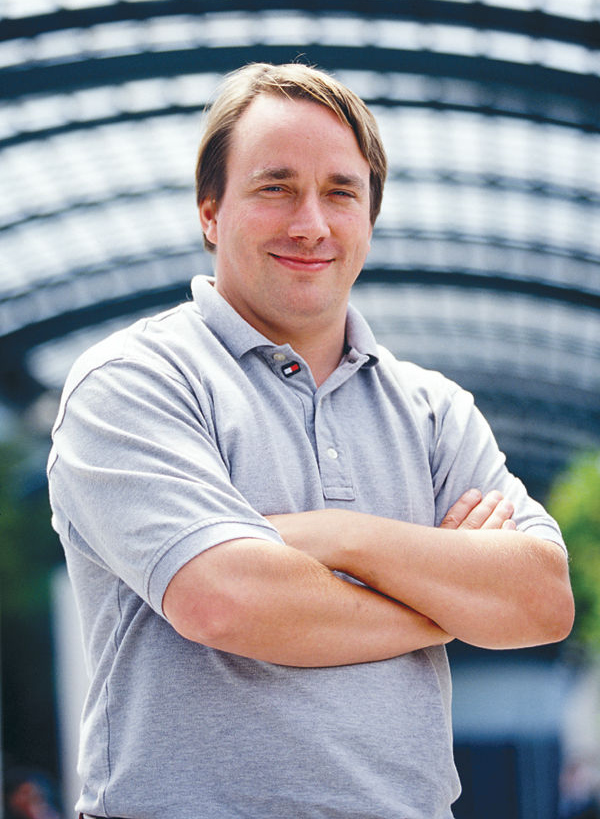
\includegraphics[width=\textwidth,height=0.8\textheight,keepaspectratio]{linus}
		\end{column}
	\end{columns}
	\blfootnote{Linus Torvalds, Linux Magazine 2002}
	
	\note[item]{
		Git is a version control system written by Linux Torvalds, the creator of Linux.
		He created it to manage the Linux kernel when the licence for the previous version control system he used was revoked.
		
		\item
		As for the name, Linus had this to say:
		``I'm an egotistical bastard, and I name all my projects after myself. First `Linux', now `git'.''
	}
\end{frame}

\subsection{Disambiguation}

\begin{frame}{Git vs GitHub}
	Git and GitHub are not the same thing!
	\medskip
	\begin{itemize}
		\item Git: version control system, runs locally
		\begin{itemize}
			\item Open source, maintained by Junio Hamano
		\end{itemize}
		\item GitHub: website and cloud server host
		\begin{itemize}
			\item Owned by Microsoft
		\end{itemize}
		\item GitLab, Bitbucket, SourceForge, etc.: other Git server hosts
	\end{itemize}
	
	\note[item]{
		This is a mistake I've heard a lot of people making, so I'm just going to clarify right now: Git and GitHub are not the same thing.
		
		\item
		Git is the version control tool.
		It's the set of commands you run on your computer.
		It's the thing originally written by Linus, and now maintained as an open source project.
		
		\item
		GitHub is a website that hosts Git repositories.
		They run a copy of Git, and serve as a place for you to store Git-managed files.
		They're not the only such host: there are dozens of commercial ones.
		You can even spin up a Git server on your own computer, and host your own.
		
		\item
		Think of Git as a file manager, and GitHub as being your friend's hard drive (or Microsoft's hard drive in this case).
		You can send files to your friend to back them up, or for them to pass on to other people.
		Meanwhile, you've still got your own copy of your file manager, and your own copy of your files.
	}
\end{frame}

\section{Motivation}

\subsection{General Use}

\begin{frame}{Why Use Git?}
	\centering
	\includegraphics[width=\textwidth,height=0.8\textheight,keepaspectratio]{phd-final}
	\blfootnote{Piled Higher and Deeper by Jorge Cham}
	
	\note[item]{
		Why do we use Git?
		The main things is that it allows us to keep different versions in a well-controlled fashion.
		It avoids the stereotypical proliferation of poorly named ``final'' versions.
		
		\item
		It's also very useful for any sort of collaborative effort.
		Have you ever done any sort of collaborative project where you're emailing files back and forth.
		Nobody can keep track of which is the most recent version.
		And if you both change a file at the same time, how do you combine the versions?
		Git handles the versioning for you, and also has a very neat algorithm for merging two sets of changes into a version with both changes.
		
		\item
		Version control is also very useful for reproducible research.
		When you share a paper, you can use version control to provide a snapshot of the code that produced it.
		Then, even if you keep working on that code, that snapshot exists for you or others to reproduce that work.
	}
\end{frame}

\subsection{Fixing Problems}

\begin{frame}{What Can Git Do?}
	\begin{itemize}
		\item What have other people changed since I last worked on this?
		\begin{itemize}
			\item \texttt{git log}
		\end{itemize}
		\item I changed some stuff, and my supervisor changed some other stuff, and I need to combine them
		\begin{itemize}
			\item \texttt{git merge}
		\end{itemize}
		\item I want to try something, but I'm worried it'll break stuff
		\begin{itemize}
			\item \texttt{git branch}
		\end{itemize}
		\item Everything I've just done has made things worse; I want to go back to how it was
		\begin{itemize}
			\item \texttt{git reset --hard} (or \texttt{git stash})
		\end{itemize}
		\item This was working fine a week ago, but now it's broken
		\begin{itemize}
			\item \texttt{git bisect}
		\end{itemize}
		\item What was I thinking when I wrote this line?
		\begin{itemize}
			\item \texttt{git blame}
		\end{itemize}
	\end{itemize}
	
	\note[item]{
		Git can do a lot more than just the standard storing and sharing of versions.
		It has a lot of benefits even just for a solo developer.
		Today, I'm going to focus mostly on just getting you working with Git.
		But next session, we'll go over some of the really helpful things you can do with it.
		
		\item
		In the meantime, here's a taste of some of the things we can do with Git.
		Have you ever found yourself in any of these situations?
		Git has commands to solve them.
	}
\end{frame}

\section{The Git Parable}

\subsection{The Parable}

\begin{frame}{How Not To Explain Git}
	\centering
	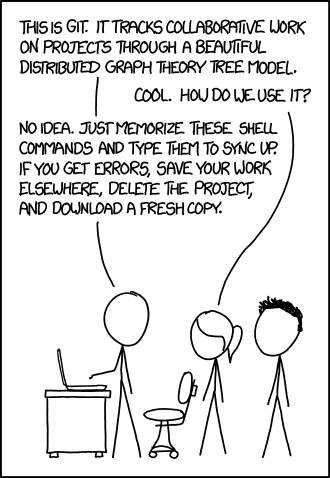
\includegraphics[width=\textwidth,height=0.8\textheight,keepaspectratio]{xkcd-git}
	\blfootnote{xkcd by Randall Munroe}
	
	\note[item]{
		A lot of people teach Git by this method: they show the standard \texttt{pull}, \texttt{add}, \texttt{commit}, \texttt{push} workflow, and leave it at that.
		The problem with doing this is that, while it allows you to work with other people who use Git, you get very little benefit from using Git that way.
		You won't understand enough to do any of the cool and useful things I just demonstrated.
	}
\end{frame}

\begin{frame}{How To Explain Git}
	The Git Parable, by Tom Preston-Werner
	\begin{itemize}
		\item \url{https://tom.preston-werner.com/2009/05/19/the-git-parable.html}
	\end{itemize}
	Suppose you only have a text editor and a file manager.
	How would you develop version control?
	
	\note[item]{
		Instead, I'm going to explain how Git actually works.
		It can appear quite complicated, so we're going to build it from the ground up.
		I'm shamelessly stealing from the best explanation of Git I've seen: ``the Git Parable'', by Tom Preston--Werner, co-founder of GitHub.
		
		\item
		The Git Parable works as follows.
		Suppose Git doesn't exist; suppose you don't have any fancy software at all.
		You've just got a text editor and a file manager, and you're setting out on a massive coding project that you need to version control.
		How, with just your text editor and file manager, would you control your versions?
	}
\end{frame}

\subsection{Snapshots}

\begin{frame}{Snapshots}
	\begin{columns}[onlytextwidth]
		\begin{column}{0.33\textwidth}
			\centering
			\includegraphics[width=\textwidth,height=0.8\textheight,keepaspectratio]{snapshot-2001-01-19}
			2001-01-19
		\end{column}
		\hfill
		\begin{column}{0.33\textwidth}
			\centering
			\includegraphics[width=\textwidth,height=0.8\textheight,keepaspectratio]{snapshot-2004-05-29}
			2004-05-29
		\end{column}
		\hfill
		\begin{column}{0.33\textwidth}
			\centering
			\includegraphics[width=\textwidth,height=0.8\textheight,keepaspectratio]{snapshot-2008-10-18}
			2008-10-18
		\end{column}
	\end{columns}
	
	\note[item]{
		Alfred is a friend of yours who works at a ``Special Moments'' photo boutique.
		He tells you the story of a woman who brings her child in for a portrait on the same day every year.
		``She brings the photos from all the past years with her,'' Alfred tells you.
		``She likes to remember what her daughter was like at each different stage, as if the snapshots really let her move back and forth in time to those saved memories.''
		
		\item
		This gives you an idea.
		Snapshots, like save points in a video game, are what you want for your version control system.
		What if you could take snapshots of your codebase at any time and resurrect that code on demand?
		So you go running back to your computer and start working.
	}
\end{frame}

\begin{frame}[t]{Snapshot Directories}
	\only<+|handout:0>{
		\dirtree{%
			.1 project.
			.2 working.
			.3 download-genomes.R.
			.3 read-genomes.R.
		}
	}
	\only<+|handout:0>{
		\dirtree{%
			.1 project.
			.2 working.
			.3 download-genomes.R.
			.3 read-genomes.R.
			.2 snapshot-0.
			.3 download-genomes.R.
			.3 read-genomes.R.
		}
	}
	\only<+|handout:0>{
		\dirtree{%
			.1 project.
			.2 working.
			.3 download-genomes.R.
			.3 read-genomes.R.
			.2 snapshot-0.
			.3 download-genomes.R.
			.3 read-genomes.R.
			.2 snapshot-1.
			.3 download-genomes.R.
			.3 read-genomes.R.
		}
	}
	\only<+>{
		\dirtree{%
			.1 project.
			.2 working.
			.3 download-genomes.R.
			.3 read-genomes.R.
			.2 snapshot-0.
			.3 message.
			.3 download-genomes.R.
			.3 read-genomes.R.
			.2 snapshot-1.
			.3 message.
			.3 download-genomes.R.
			.3 read-genomes.R.
		}
	}
	
	\note[item]{
		You begin with a \texttt{project} directory.
		This will contain everything for the project, including all your versions.
		
		\item
		Within this, you create a \texttt{working} directory.
		This will contain all the code, however many files that is.
		This is the version you'll change as you work.
		
		\item
		When you've a written a feature, you make sure everything's saved, then copy the entire \texttt{working} directory to \texttt{snapshot-0}.
		You make sure never to change any of the files in \texttt{snapshot-0}; they're permanently fixed.
		You keep making changes in \texttt{working}, and when you're done with the next feature, you again copy the whole of \texttt{working} to \texttt{snapshot-1}.
		
		\item
		These numbers aren't very helpful, so you create a file called \texttt{message} in each snapshot directory.
		This records the date of creation, and a summary of the work you did in that snapshot.
	}
\end{frame}

\begin{frame}[fragile]{Commit Messages}
	\texttt{snapshot-0/message}
	\begin{lstlisting}[frame=single,tabsize=4,gobble=8]
		2023-08-13T11:02:29+10:00
		Add download() to download FASTA files.
	\end{lstlisting}
	\bigskip
	\texttt{snapshot-1/message}
	\begin{lstlisting}[frame=single,tabsize=4,gobble=8]
		2023-08-13T11:27:47+10:00
		Refactor download() to use web_history.
		
		This should allow larger values of retmax,
		speeding up the download.
	\end{lstlisting}
	
	\note[item]{
		The message files for a couple of snapshots might look like this, with a date and time of creation, and a summary of what work was done to create them.
		
		\item
		I've written the date and time in ISO format: year, month, day, 24 hour time, and time zone offset.
		Git actually stores them in UNIX format: the number of seconds since the beginning of 1970, plus time zone offset.
		But that's not human readable.
		
		\item
		Note that each snapshot represents a single, small unit of work.
		Per Git convention, I've written the summary messages in the imperative tense: ``do this''.
		We can use extra lines to provide extra information, such as the justification for a change.
	}
\end{frame}

\subsection{Branches}

\begin{frame}[t]{Non-Linear Development}
	\only<+|handout:0>{
		\dirtree{%
			.1 project.
			.2 working.
			.2 snapshot-0.
			.2 ....
			.2 snapshot-99.
		}
	}
	\only<+|handout:0>{
		\dirtree{%
			.1 project.
			.2 working.
			.2 snapshot-0.
			.2 ....
			.2 snapshot-99.
			.2 ....
			.2 snapshot-109.
		}
	}
	\only<+>{
		\dirtree{%
			.1 project.
			.2 working.
			.2 snapshot-0.
			.2 ....
			.2 snapshot-99.
			.2 ....
			.2 snapshot-109.
			.2 snapshot-110\hspace{0.5em}\textrm{?}.
		}
	}
	\note[item]{
		So, you now have a version control system, and it's working great.
		You can jump back to any earlier version whenever you want.
		
		\item
		You keep making changes, and making snapshots, and eventually you get to \texttt{snapshot-99}.
		Happy with what you've got, you release \texttt{snapshot-99} to the general public, as release version 1.0.
		
		\item
		The public likes your software, so you set out to add new features for the next version.
		You create another ten snapshots, and soon you're at \texttt{snapshot-109}.
		
		\item
		But then the bug reports start rolling in.
		It's fine, nobody's perfect, but it turns out that people using \texttt{snapshot-99} have found some problems.
		You don't want all your new features getting in the way while you debug, so you copy the contents of \texttt{snapshot-99} into your \texttt{working} directory.
		It's a quick fix, and soon you're ready to create \texttt{snapshot-110}.
		But now you've got a problem.
		\texttt{snapshot-110} is based on \texttt{snapshot-99}, not \texttt{snapshot-109}.
	}
\end{frame}

\begin{frame}{Branches}
	\begin{columns}[onlytextwidth]
		\begin{column}{0.6\textwidth}
			\centering
			\includegraphics[width=\textwidth,height=0.75\textheight,keepaspectratio]{tree}
			\blfootnote{Winter Tree, Haslemere, by Simon Burchell}
		\end{column}
		\hfill
		\begin{column}{0.4\textwidth}
			\centering
			\newcommand\treediagram{
				\graph[tree layout,grow'=up,fresh nodes] { %fresh nodes allows duplicate node names.
					snapshot0/"snapshot-0" <- "\rvdots" <- snapshot99/"snapshot-99" <- {
						snapshot100/"snapshot-100" <- "\rvdots" <- snapshot109/"snapshot-109",
						snapshot110/"snapshot-110"
					}
				};
			}
			\begin{tikzpicture}[>={Stealth[length=4pt,width=4pt]}]
				\treediagram
			\end{tikzpicture}
		\end{column}
	\end{columns}
	
	\note[item]{
		Pondering the problem, you decide to go for a walk in nature.
		Your eyes fall upon a large tree beside the path.
		Fixing your gaze upon one twig, it's easy easy to follow it back to the base of the tree.
		From the twig to the branch it grew from, from branch to bough, bough to trunk, and then down to the roots.
		
		\item
		You realise this is the perfect model for keeping trach of multiple lines of development.
		For each snapshot, you just need to keep track of which snapshot it grew from, and then following these links, you will be trace any branch right back to the root, following the whole line of development.
	}
\end{frame}

\begin{frame}[fragile]{Parents}
	\texttt{snapshot-99/message}
	\begin{lstlisting}[frame=single,tabsize=4,gobble=8]
		parent snapshot-98
		2023-08-20T09:15:16+10:00
		Update version number to 1.0.0.
	\end{lstlisting}
	
	\texttt{snapshot-100/message}
	\begin{lstlisting}[frame=single,tabsize=4,gobble=8]
		parent snapshot-99
		2023-08-21T01:00:12+10:00
		Add query() to get a list of available files.
	\end{lstlisting}
	
	\texttt{snapshot-110/message}
	\begin{lstlisting}[frame=single,tabsize=4,gobble=8]
		parent snapshot-99
		2023-08-22T06:29:05+10:00
		Fix download() failing on Windows machines.
	\end{lstlisting}
	
	\note[item]{
		So, how do you implement this?
		Simple: store the parent of each snapshot in the \texttt{message} file.
		
		\item
		This is what it might look like.
		Each \texttt{message} file now has an extra line, giving the parent.
		For now, most snapshots just use the previous number as the parent: 99's parent is 98, 100's parent is 99.
		But the parent of snapshot 110 is snapshot 99.
		
		\item
		Just this simple mecahnism suffices to store the entire structure of the tree, and the entire history for any snapshot.
	}
\end{frame}

\begin{frame}{Branch Names}
	\centering
	\begin{tikzpicture}[>={Stealth[length=4pt,width=4pt]},node distance=1em]
		\onslide<+->{
			\graph[tree layout,grow'=up,fresh nodes] { %fresh nodes allows duplicate node names.
				snapshot0/"snapshot-0" <- "\rvdots" <- snapshot99/"snapshot-99" <- {
					snapshot100/"snapshot-100" <- "\rvdots" <- snapshot109/"snapshot-109",
					snapshot110/"snapshot-110"
				}
			};
		}
		\onslide<+->{
			\node[branch,right=of snapshot109] (master) {master} edge[->,branch] (snapshot109);
			\node[branch,right=of snapshot110] (v1maintenance) {v1.0-maintenance} edge[->,branch] (snapshot110);
		}
		\onslide<+->{
			\node[tag,right=of snapshot99] (v1) {v1.0.0} edge[->,tag] (snapshot99);
		}
	\end{tikzpicture}
	
	\note[item]{
		So, the code history is now a tree, and we can trace any snapshot back to the root.
		This is great; we can now have multiple lines of development at once.
		
		\item
		But there's a problem.
		If we're just looking at the list of all snapshots, how do we know which is the most recent one on each branch?
		It was fine when they were sequential: the highest number was the most recent.
		But what about now?
		
		\item
		So, we need to keep a list of the most recent snapshot for each branch.
		This is a list of pointers to snapshots, one for each branch.
		We've got two branches now.
		The one we're mostly working on and developing new features on, we'll call \texttt{master}.
		The one for fixing bugs in the release version, we'll call it \texttt{v1.0-maintenance}.
		
		\item
		While we're at it, it'd be nice to keep track of some other important snapshots, like the \texttt{snapshot-99} that we released to the public.
		We'll point at this one, and call it \texttt{v1.0.0}.
	}
\end{frame}

\begin{frame}[fragile]{Storing Branches}
	\texttt{branches}
	\begin{lstlisting}[frame=single,tabsize=4,gobble=8]
		master snapshot-109
		v1.0-maintenance snapshot-110
	\end{lstlisting}
	\bigskip
	\texttt{tags}
	\begin{lstlisting}[frame=single,tabsize=4,gobble=8]
		v1.0.0 snapshot-99
	\end{lstlisting}
	
	\note[item]{
		So, how will we store these branch pointers.
		We'll create a special file called \texttt{branches}.
		\texttt{branches} doesn't sit in \texttt{working}, or in any of the snapshots.
		It's got to live somewhere separate.
		In this parable, we'd keep it in the top level project directory.
		In practice, Git keeps it in a special \texttt{.git} directory.
		
		\item
		So we just have a file listing each branch, and which snapshot is its tip.
		Whenever we create a new snapshot on the end of a branch, we need to update this file.
		
		\item
		The other special snapshots, we'll call ``tags'', and we'll put them in another file (also called \texttt{tags}).
		Tags are exactly like branches, except that they never move.
		That snapshot will always have been the v1.0.0 release.
		
		\item
		A note:
		\texttt{master} is the default name Git will use for the first branch when you create a repository, but there's nothing special about it.
		GitHub has recently been encouraging people to call it \texttt{main} instead.
	}
\end{frame}

\subsection{Distributed}

\begin{frame}{A Sharing Problem}
	\centering
	\begin{tikzpicture}[>={Stealth[length=4pt,width=4pt]},subgraph text top=text centered,subgraph nodes={font=\bfseries}]
		\graph[fresh nodes,tree layout,grow'=up] {
			you/You[draw] // {
				snapshot0/"snapshot-0" <- "\rvdots" <- snapshot111/"snapshot-111" <- {
					snapshot112/"snapshot-112" <- snapshot114/"snapshot-114" <- snapshot115/"snapshot-115",
					snapshot113/"snapshot-113"
				}
			},
			zoe/Zoe[draw] // {
				snapshot0/"snapshot-0" <- "\rvdots" <- snapshot111/"snapshot-111" <- {
					snapshot112/"snapshot-112",
					snapshot113/"snapshot-113" <- snapshot114/"snapshot-114" <- snapshot115/"snapshot-115"
				}
			}
		};
	\end{tikzpicture}
	
	\note[item]{
		So far, you've been working by yourself.
		But that gets lonely.
		Thankfully, you've got a friend called Zoe, adn she wants to help you.
		You're liking your version control system, so you send her the whole thing.
		You just email her the entire project directory, working, snapshots, branches and tags files, and all.
		Then Zoe catches a flight to Patagonia and you don't hear from her for a week.
		
		\item
		When she gets back, you notice a problem.
		You've both been coding, and making new snapshots.
		But you're both using the same numbering system, so now you both have snapshots called \texttt{snapshot-114}, \texttt{snapshot-115}, etc.\ but with different code in them.
		You can't copy her snapshots without overwriting yours.
		And even if you could, you'd have no idea who wrote which code.
	}
\end{frame}

\begin{frame}[fragile]{Attributing Blame}
	\texttt{snapshot-114/message}
	\begin{lstlisting}[frame=single,tabsize=4,gobble=8]
		parent snapshot-110
		Christopher Brown <pyrrhicpachyderm@gmail.com>
		2023-08-22T13:09:24+10:00
		Retry downloads on 5xx HTTP errors.
		
		HTTP error codes 500 to 511 are failures on
		valid requests. They may occur erratically,
		so just retry the download.
	\end{lstlisting}
	
	\note[item]{
		Not knowing who wrote what is thankfully easy to solve.
		You add the author's name and email address to every \texttt{message} file.
	}
\end{frame}

\begin{frame}[fragile]{The Return of Hashing}
	\texttt{6d97fcee39f983edc17e304db8381ad3174c15d9/message}
	\begin{lstlisting}[frame=single,tabsize=4,gobble=8]
		Christopher Brown <pyrrhicpachyderm@gmail.com>
		2023-08-13T11:02:29+10:00
		Add download() to download FASTA files.
	\end{lstlisting}
	\medskip
	\texttt{edd9a01a7b0255754b07e57055cafd3f3cdea3b5/message}
	\begin{lstlisting}[frame=single,tabsize=4,gobble=8]
		parent 6d97fcee39f983edc17e304db8381ad3174c15d9
		Christopher Brown <pyrrhicpachyderm@gmail.com>
		2023-08-13T11:27:47+10:00
		Refactor download() to use web_history.
		
		This should allow larger values of retmax,
		speeding up the download.
	\end{lstlisting}
	
	\note[item]{
		The other problem---two snapshots having the same name---is more troublesome.
		Thankfully, you recently learned about hashing (remember that?), and you realise it presents the answer to your problems!
		Instead of calling a snapshot \texttt{snapshot-0}, you hash its \texttt{message} file, and use the hash of that as the snapshot name.
		
		\item
		Here, we've done this to the first two snapshots, previous \texttt{snapshot-0} and \texttt{snapshot-1}.
		The first \texttt{message} file hashes to give the string that forms the new snapshot name.
		We then use this snapshot name as the parent for the next snapshot, and hash that, \texttt{message} to get the name for that snapshot.
		
		\item
		Remember how a hash changes totally if any part of the contents changes?
		So two snapshots will only get the same name if they're created at the same time, by the same person, with the same summary.
	}
\end{frame}

\begin{frame}{Recombining}
	\centering
	\begin{tikzpicture}[>={Stealth[length=4pt,width=4pt]},subgraph text top=text centered,subgraph nodes={font=\bfseries}]
		\graph[fresh nodes,tree layout,grow'=up] {
			you/You[draw] // {
				6d97fce <- "\rvdots" <- 2de04ad <- {
					4b36dc9 <- 2138c74 <- 367d5d5,
					2a2b6cf
				}
			},
			combined/Combined[draw] // {
				6d97fce <- "\rvdots" <- 2de04ad <- {
					4b36dc9 <- 2138c74 <- 367d5d5,
					2a2b6cf <- 3603f71 <- 2a2b6cf
				}
			},
			zoe/Zoe[draw] // {
				6d97fce <- "\rvdots" <- 2de04ad <- {
					4b36dc9,
					2a2b6cf <- 3603f71 <- 2a2b6cf
				}
			}
		};
		\path (you) edge[->,red] (combined);
		\path (zoe) edge[->,red] (combined);
	\end{tikzpicture}
	
	\note[item]{
		Now that you and Zoe have renamed all your snapshots, you can merrily combine your repositories, because none of her snapshots have the same name as any of yours.
		You can just copy all of her snapshots into your \texttt{project} directory, and vice versa, and there won't be any collisions or confusion; you'll both have a copy of one another's work.
		
		\item
		This point is important, so it's worth reiterating.
		The hash of a snapshot uniquely identifies it (and its parent).
		Thus, entire snapshots can be passed around between different computers without losing their identity, or their place in the history tree.
	}
\end{frame}

\begin{frame}{Distributed}
	Advantages of a distributed system:
	\begin{itemize}
		\item Can work offline
		\item Can keep things private
		\item No single point of failure
	\end{itemize}
	
	\note[item]{
		Note that this is a distributed system.
		Everybody has their own copy of the repository.
		There are a number of advntages to this, over the centralised systems that some other version control systems use.
		
		\item
		You can do all your work offline.
		Zoe spends a lot of time flying around to different countries, with spotty internet access, so she appreciates this.
		it also makes things much faster, 'cause you don't need to talk to a server every time you want to do something.
		You only need the internet to share your work.
		
		\item
		You can also choose to keep some of your work private.
		Everything's fine if you decide not to share certain snapshots or branches with Zoe.
		
		\item
		Note that we haven't invoked GitHub here.
		You and Zoe can keep emailing snapshots to one another, with no need for a central host.
		But if you do use GitHub, it doesn't matter if GitHub goes bankrupt and vanishes.
		Everyone's got a copy, so everyone's got a backup.
	}
\end{frame}

\end{document}
